\documentclass[12pt, letterpaper]{article}

\setlength {\marginparwidth }{2cm}

\usepackage{tikz}
\usetikzlibrary{shapes,arrows}
\tikzstyle{line}=[draw]
\usepackage{amsthm}
\usepackage{amsmath}
\usepackage[textsize=tiny]{todonotes}
\usepackage{array}
\newcolumntype{L}{>$l<$}

%\newtheorem{thm}{Theorem}
%\newtheorem{defn}[thm]{Definition}

\newtheorem{thm}{Theorem}
\newtheorem{lem}[thm]{Lemma}
\newtheorem{defn}[thm]{Definition}
\newtheorem{ex}[thm]{Example}
%\newtheorem{claim}[thm]{Claim}

\newcommand{\squash}{\parskip=0ex\itemsep=0ex}
\newcommand{\cnf}[1]{\ensuremath{\operatorname{\mathsf{#1}}}}
\newcommand{\cnc}[1]{\ensuremath{\mathsf{#1}}}
\newcommand{\fnf}[1]{\ensuremath{\operatorname{\mathit{#1}}}}
\newcommand{\fnc}[1]{\ensuremath{\mathit{#1}}}

% Binary operators for linear and branching terms
\newcommand{\linseq}{\prec}
\newcommand{\linpar}{\sim}
\newcommand{\sdup}{\leftrightarrow}
\newcommand{\slft}{\leftarrow}
\newcommand{\srht}{\rightarrow}
\newcommand{\bradupseq}{\stackrel{\sdup}{\linseq}}
\newcommand{\bralftseq}{\stackrel{\slft}{\linseq}}
\newcommand{\brarhtseq}{\stackrel{\srht}{\linseq}}
\newcommand{\braduppar}{\stackrel{\sdup}{\linpar}}
\newcommand{\bralftpar}{\stackrel{\slft}{\linpar}}
\newcommand{\brarhtpar}{\stackrel{\srht}{\linpar}}
\newcommand{\linseqe}{\to}
\newcommand{\braseqe}[1]{\stackrel{#1}{\prec}}
\newcommand{\brapare}[1]{\stackrel{#1}{\sim}}

\newcommand{\apdt}{APDT}
\newcommand{\skp}{\cnc{SKIP}}
\newcommand{\cpy}{\cnc{CPY}}
\newcommand{\done}{\cnc{DONE}}
\newcommand{\at}[2]{\mathop{@_{#1}}{#2}}
%\newcommand{\ati}[3]{\mathop{@_{#1}}[{#2}]{#3}}
\newcommand{\sig}{\cnc{SIG}}
\newcommand{\hsh}{\cnc{HSH}}
\newcommand{\kimc}{\cnc{KIM}}
\newcommand{\kim}[3]{\cnc{KIM}~#1~#2~#3}
\newcommand{\kime}[3]{\cnc{KIM}~#1~#2~#3}
\newcommand{\usm}{\cnc{USM}}
\newcommand{\usme}[2]{\cnc{USM}~#1~#2}

\newcommand{\seqe}{\mathbin{;\!;}}
\newcommand{\pare}{\parallel}
\newcommand{\mt}{\xi}
%\newcommand{\sign}[2]{[\![#1]\!]_{#2}}
\newcommand{\hash}[2]{\mathop{\#_{#1}}{#2}}
\newcommand{\KK}[2]{\cnc{K}^{#1}_{#2}}
\newcommand{\UU}[1]{\cnc{U}_{#1}}
\newcommand{\Ke}[4]{\cnc{K}^{#1}_{#3}({#4})}
\newcommand{\Ue}[3]{\cnc{U}_{#2}({#3})}
\newcommand{\Ne}[2]{\cnc{N}_{#1}({#2})}

\newcommand{\eval}[3]{\mathcal{E}({#1},{#2},{#3})}
\newcommand{\aeval}[3]{\bar{\mathcal{E}}({#1},{#2},{#3})}
\newcommand{\evalS}[1]{\ensuremath{\mathcal{E}(#1)}}
\newcommand{\evalv}[3]{\mathcal{V}({#1},{#2},{#3})}
\newcommand{\evalvS}[1]{\mathcal{V}({#1})}
\newcommand{\po}[3]{\mathcal{R}({#1},{#2},{#3})}
\newcommand{\bfr}[3]{{#1}\mathbin:{#2}\prec{#3}}
%\newcommand{\bfr}[3]{{#2}\prec_{#1}{#3}}
\newcommand{\splt}[2]{\mathcal{S}({#1},{#2})}
\newcommand{\subterm}{\sqsubseteq}
\newcommand{\sevalf}{\mathcal{F}}
\newcommand{\seval}[1]{\sevalf({#1})}
\newcommand{\placef}{\mathcal{G}}
\newcommand{\place}[1]{\placef({#1})}
\newcommand{\halt}[1]{\mathcal{H}({#1})}
\newcommand{\size}[1]{|{#1}|}
\newcommand{\evof}{\mathrel\Diamond}
\newcommand\te[4]{{#1}\evof^{#2}_{#3}{#4}}
% for tables
\newcommand\tte[4]{{#1}&{}\evof^{#2}_{#3}{}&{#4}}

\newcommand{\futr}{\cnc{FUTR}}

\newcommand{\nat}{\mathbb{N}}
\newcommand{\anno}[3]{[{#1}]^{#2}_{#3}}
\newcommand{\step}{\leadsto}
\newcommand{\lts}[3]{{#2}\mathbin:{#1}\step{#3}}
\newcommand{\lstp}[3]{{#1}\stackrel{#2}{\leadsto}{#3}}
\newcommand{\nstep}[1]{\leadsto^{{}_{#1}}}
\newcommand{\kstar}{\leadsto^*}
\newcommand{\nlstep}[2]{\stackrel{\!\!#1}{\leadsto^{{}_{#2}}}}
\newcommand{\lstep}[1]{\stackrel{#1}{\leadsto}}
\newcommand{\lstar}[1]{\stackrel{\!\!#1}{\leadsto^{{}_{*}}}}
\newcommand{\nlstar}[2]{\stackrel{\!\!#1}{\leadsto^{{}_{#2}}}}
\newcommand{\sseq}{\mathbin{;}}
\newcommand{\sfut}{\mid}
\newcommand{\qmid}{\mathbin{\mbox{`$\mid$'}}}
\newcommand{\ssft}{\mathbin{;\!;}}
\newcommand{\spar}{\parallel}
\newcommand{\sstop}{\mathcal{D}}
\newcommand{\conf}{\mathcal{C}}
\newcommand{\lseq}{\mathcal{LS}}
\newcommand{\bseq}{\mathcal{BS}}
\newcommand{\bpar}{\mathcal{BP}}
\newcommand{\ats}{\mathcal{A}}

\newcommand{\compf}{\mathcal{C}}
\newcommand{\comp}[2]{\compf({#1},{#2})}
\newcommand{\compp}[2]{[{#2}]_{#1}}
\newcommand{\cop}[1]{\mathbin{\cdot{#1}\cdot}}
\newcommand{\atc}[1]{\mathop{\bar{@}_{#1}}}
\newcommand{\estep}{\Rightarrow}

\newcommand{\seq}[1]{\ensuremath{\langle#1\rangle}}
%\newcommand{\app}{\mathbin{{}^\smallfrown}}
\newcommand{\app}{\mathbin{\ast}}
\newcommand{\cons}{\mathbin{::}}
\newcommand{\sel}{\mathbin{\downarrow}}

\newcommand{\csize}[1]{\ensuremath{\mid\!#1\!\mid}}
\newcommand{\labi}[2]{\ensuremath{\alpha({#1},#2)}}
\newcommand{\lab}[1]{\ensuremath{\alpha(#1)}}
%\newcommand{\tsize}[1]{\ensuremath{\mid\!#1\!\mid}}
\newcommand{\tsize}[1]{\size{#1}}

\newcommand{\term}{\cnc{APDT}}
%\newcommand\tr[4]{{#1}\mathcal{T}^{#2}_{#3}{#4}}
\newcommand\tr[4]{{#1}\mathbin\Box^{#2}_{#3}{#4}}
\newcommand{\trace}[2]{\ensuremath{\mathcal{T}(#1,#2)}}
\newcommand{\traceS}[2]{\ensuremath{\mathcal{T}(#1,#2)}}


\newcommand{\utype}[3]{\cnc{(\forall#1<:#2.\hspace{1mm} #3)}}
\newcommand{\tyu}[2]{\cnc{(\forall#1.\hspace{1mm} #2)}}
\newcommand{\uterm}[3]{\cnc{(\lambda#1<:#2.\hspace{1mm} #3)}}
\newcommand{\nilenv}[0]{$\emptyset$}
\newcommand{\topt}{\cnc{TOP}}
\newcommand{\noncec}{\cnc{NONCE}}
\newcommand{\lam}[3]{\cnc{(\lambda}#1:#2 . \hspace{1mm} #3)}
\newcommand{\tylam}[2]{\cnc{(\lambda}#1 . \hspace{1mm} #2)}
\newcommand{\typest}[0]{\cnc{T} }
\newcommand{\id}[0]{\cnc{\emph{x}} }
\newcommand{\tid}[0]{\cnc{\emph{X}} }
\newcommand{\appl}[2]{#1 \hspace {2mm} #2}
\newcommand{\tappl}[2]{#1 \hspace {2mm} [#2]}
%%\newcommand{\terms}[0]{\cnc{\emph{t}} }
\newcommand{\meast}[0]{\cnc{MEAS}}
\newcommand{\evt}[0]{\cnc{\emph{E}} }
\newcommand{\evc}[0]{\cnc{\emph{e}} }
\newcommand{\arrt}[2]{#1 \hspace{1mm} \cnc{\rightarrow} \hspace{1mm} #2}
\newcommand{\pl}[0]{\cnc{\emph{P}} }
\newcommand{\placec}[1]{\cnc{pl_#1}}
\newcommand{\placee}[1]{\cnc{PL_#1}}
\newcommand{\placet}[0]{\cnc{PLACE_Q}}
\DeclareMathOperator{\vvdash}{\vdash}
\newcommand{\typeof}[3]{\cnc{\Gamma \vvdash\limits_{#1,#2} : #3}}
\newcommand{\btt}[2]{\cnc{(#1,#2)} \hspace{1mm} \ensuremath{\epsilon\hspace{1mm}\Gamma}}
\newcommand{\bs}{\cnc{BS}}
\newcommand{\argt}{\cnc{ARG}}
\newcommand{\Uec}[5]{\cnc{U}_{#1}~#2~#3~#4~(#5)}
\newcommand{\Kec}[6]{\cnc{K}^{#1}_{#2}~#3~#4~#5~(#6)}
\newcommand{\Gec}[3]{\cnc{G}_{#1} \hspace{1mm} #2 \hspace{1mm}  #3}
\newcommand{\Hec}[2]{\cnc{H}_{#1} \hspace{1mm} #2}
\newcommand{\Nec}[3]{\cnc{N}_{#1} \hspace{1mm} #2 \hspace{1mm} (#3)}
\newcommand{\Sec}[2]{\cnc{SS} \hspace{1mm} {#1} \hspace{1mm} {#2}}
\newcommand{\Pec}[2]{\cnc{PP} \hspace{1mm} {#1} \hspace{1mm} {#2}}
\newcommand{\mtc}{\cnc{mt}}
\newcommand{\strj}{\cnc{<string>}}
\newcommand{\numj}{\cnc{<number>}}
\newcommand{\arrj}{\cnc{<array>}}
\newcommand{\tj}{\cnc{<term>}}
\newcommand{\ej}{\cnc{<evidence>}}
\newcommand{\namej}{\cnc{<nameMap>}}
\newcommand{\reqmc}[5]{#1~#2~#3~#4~#5}
\newcommand{\respmc}[4]{#1~#2~#3~#4}

\newcommand{\squash}{\itemsep=0pt\parskip=0pt}

\title{Context Relation Musings}
\author{Anna Fritz}
\date{\today}

\begin{document}

\maketitle

\section{Context Defined}

First, in order to do any real reasoning about a system's context, we must formally define it. 

\begin{defn}[Context]
  A system's \emph{context} is a relationship represented within a Manifest that describes the dependencies within the system. 
\end{defn}

Some questions and interesting points arise when attempting to grasp this definition and realize the following example. Below are some words I think we need to define as we work towards the ordering problem. 

Correctly defining a dependency is critical as we need to capture the intricacies of a layered system. We want to take bottom up measurements for many reasons, one being to confine an adversary \cite{Rowe::Bundling}.

\begin{defn}[Dependency] 
  One component \emph{depends} on another when... 
\end{defn}

\begin{defn}[Separation] 
  \emph{Separation} between components within the system is realized when... (this definition is motivated by \cite{Ramsdell::Orchestrating} )
\end{defn}

\begin{defn}[Similar] 
  One protocol is \emph{similar} to another when... They measure the same targets? The measurement chain reaches the same depth? The measurement chain reaches the same range? .. consider defining "similar" as a weak bisimulation
\end{defn}

\begin{defn}[Better] 
  One protocol is \emph{better} than another when... consider better as the top of the lattice or the "highest" protocol in the preorder. 
\end{defn}

\begin{defn}[Trust Chain]
  A emph{trust chain} is a measurement chain that begins at the root of trust and proceeds by taking measurements of the next closest layer until the top layer is measured thereby producing a layered attestation. 
\end{defn}

\section{Mathematics}

Here are some interesting mathematically defined structures that could be useful. 

\begin{defn}[(Labeled) Transition System]
  A \emph{transition system} is a triple $<S,S_0, \linseqe>$, with a set of states S, a set of initial states $S_0 \subseteq S$, and a transition relation $\linseqe \subseteq S \times S$ \cite{FRAP}
\end{defn}

I believe this definition raises many questions. What is the initial state? What are the set of state? What is the transition relation? A state could be some atomic action and a transition relation could be any control flow action. Another thought is only the $\at{}{}$ operator is a transition relation as it transfers the data and control from one plate to another. These questions are all answered below in the Transition System section. 

Related to a transition system, we could define \emph{reachable}, an \emph{invariant}, and possibly some \emph{correctness} condition. Recall from class, an invariant is a property that is true in all states. A state is reachable if there is some starting state from which we can transition to the reachable state. 

We may want to reason about protocol behavior to say that if two protocols produce the same evidence, then they are behaviorally equivalent. To do this, we may need to use a weak bisimulation. 

\begin{defn}[Weak Bisimulation]
A weak bisimulation is a relation \textbf{R} such that P \textbf{R} Q $\implies$ $\forall \mu, P, P' (P \xrightarrow[]{\mu} P' \implies \forall Q'. Q \overset{\mu}\Rightarrow Q'$ and P' \textbf{R} Q' ) \cite{Milner} 
\end{defn}

This says if we have some relation that relates P and Q and we can take some step from P to P' through $\mu$ and some potentially different steps from Q to Q' but again through $\mu$ then P' is related to Q'.  \todo{this doesn't seem right?}

\begin{defn}[Partially Ordered Set]
  A partially ordered set $(E, \preceq)$ is defined by it's underlying set E and it's ordering relation $\preceq$
\end{defn}

Consider \emph{upper bound} and emph{lower bound} of the poset for possible interesting properties. 

\todo{define our ordering relation. Maybe its ordered by dependencies?}

\section{Example System}

Consider the example presented in Figure \ref{fig:Host1} where a request is sent to a target $Host1$. We know a request is a list of protocols as Copland phrases. Let's assume that $R$ = [ $\at{Host1}{} $ (ASP Host2 t2) ] which says some relying party would like the target system to preform a measurement of the target $T2$ located on $Host2$. 

The arrow between ASP and T2 reveals that ASP can measure T2. This results in the following Copland phrase: 

\begin{center}
  $ \at{Host1} (ASP\:\: Host2\:\: T2)$
\end{center}

\begin{figure}[hbtp]
  \centering \begin{tikzpicture}[->,>=stealth']

      \node (req) at (-8,0) {Request};
  
      \node[rectangle,
            draw,
            fill = yellow!30,
            minimum width = 5cm, 
            minimum height = 5cm] (r) at (-3,0) {};
      \node[anchor=south] at (r.south) {Host1};
      
      \node[rectangle,
            draw,
            fill = orange!30,
            minimum width = 3.5cm, 
            minimum height = 3.5cm] (AM) at (r.center) {};
      \node[anchor=south] at (AM.south) {AM}; 

      \node[rectangle,
            draw,
            fill = white,
            minimum width = 1cm, 
            minimum height = 1cm] (ASP) at (-3.5,0) {};
      \node at (ASP.center) {ASP};

      \node[rectangle,
            draw,
            fill = white,
            minimum width = 1cm, 
            minimum height = 1cm] (T1) at (-2,0) {};
      \node at (T1.center) {T1};

      \node[rectangle,
            draw,
            fill = blue!30,
            minimum width = 3cm, 
            minimum height = 4cm] (Host2) at (3,0) {};
      \node[anchor=south] at (Host2.south) {Host2}; 

      \node[rectangle,
            draw,
            fill = white,
            minimum width = 1cm, 
            minimum height = 1cm] (T2) at (3,0) {};
      \node at (T2.center) {T2};
      

      \path[every node/.style={font=\sffamily\small}]
      (req) edge node [right] {} (r.west)
      (ASP.east) edge node [right] {} (T1.west)
      (ASP.east) edge[bend left = 90] node [left] {} (T2.west);

      % \draw (ASP.east) -- (T1.west); 
      % \draw [bend right] (ASP.east) -- (T2.west); 
  
  \end{tikzpicture}
  \caption{Example Target System.}
  \label{fig:Host1}
\end{figure}

For examples sake, say that ASP no longer has direct access to the measurement target T2 yet the goal of the attestation was to measure T2. This means we will have to realize a measurement of T2 is a different way. To start, we can expand Host2 to get a view of its attestation capabilities. This is represented with Figure \ref{fig:Host2}. We see Host2 has some ASP, $ASP2$ which can preform a measurement of $T2$. The integrity of the measurer $ASP2$ depends on the integrity of the following components: the operating system (OS), the device driver (DR), and some cryptographic operations $ \{ \}_{K}$. Then, these components all depend on the integrity of the root of trust measurement (RoTM). These dependencies are represented within Host2's manifest. 

In an abstract-ish version of Copland, the measurement chain for HOST2 could look like: 

\begin{center}
  $ \at{Host2}{(ROTM \linseqe ( OS \brapare{} DR \brapare{} \{ \}_{K} ) \linseqe (ASP2\:\: Host2\:\: T2))}$
  \todo{I have no idea how to use parathesis and Copland...}
\end{center}

where $\linseqe$ represents sequenced measurement and $\brapare{}$ represents parallel measurement. In other words, this phrase says, measure the root of trust, then measure OS, DR, and $\{ \}_{K}$ in parallel, then finally use ASP2 to take a measurement of T2. 

\todo{To be technically correct, how do you phrase the relationship between OS, DR, and SIG and the ROTM?}

\begin{figure}[]
  \centering \begin{tikzpicture}[->,>=stealth']

    \node[rectangle,
          draw,
          fill = blue!30,
          minimum width = 4cm, 
          minimum height = 4cm] (Host2) at (0,0) {};
    \node[anchor=north] at (Host2.north) {Host2}; 

    \node[rectangle,
          draw,
          fill = white,
          minimum width = 1cm, 
          minimum height = 1cm] (T2) at (0,.5) {};
    \node at (T2.center) {T2};

    \node[rectangle,
        draw,
        fill = white,
        minimum width = 1.3cm, 
        minimum height = 1cm] (ASP2) at (0,-1) {};
    \node at (ASP2.center) {ASP2};

    \node[rectangle,
        draw,
        fill = white,
        minimum width = 1cm, 
        minimum height = 1cm] (OS) at (-2,-3) {};
    \node at (OS.center) {OS};

    \node[rectangle,
        draw,
        fill = white,
        minimum width = 1cm, 
        minimum height = 1cm] (DR) at (0,-3) {};
    \node at (DR.center) {DR};

    \node[rectangle,
        draw,
        fill = white,
        minimum width = 1cm, 
        minimum height = 1cm] (SIG) at (2,-3) {};
    \node at (SIG.center) {$ \{ \}_{K}$};

    \node[rectangle,
        draw,
        fill = green!30,
        minimum width = 2cm, 
        minimum height = 1cm] (RoTM) at (0,-5) {};
    \node at (RoTM.center) {ROTM};
    

    \path[every node/.style={font=\sffamily\small}]
    (ASP2.north) edge node [left] {} (T2.south)
    (OS.north) edge [dotted] node {} (ASP2.south)
    (DR.north) edge [dotted] node {} (ASP2.south)
    (SIG.north) edge [dotted] node {} (ASP2.south)
    (RoTM.north) edge node {} (OS.south)
    (RoTM.north) edge node {} (DR.south)
    (RoTM.north) edge node {} (SIG.south);

\end{tikzpicture}
  \caption{Example Host2 System.}
  \label{fig:Host2}
\end{figure}

For examples sake, say that ASP no longer has access to the measurement of T2 directly yet the goal of the attestation is to measure T2. Combining Host1 and Host2 and representing this new fact, we have the following system in Figure \ref{fig:System1}. If the request remains \\  $R$ = [ (ASP Host2 T2) ] we must consider what would be a ``similar'' measurement? This idea captures the concept of ordering measurements using the \emph{measures} and \emph{context} relations. 

\todo{define similar?}

\pagebreak
Say we have the following protocol, as would be represented in Figure \ref{fig:Host1} and Figure \ref{fig:Host2}.

\begin{eqnarray*}
  P1 &=& \at{Host1} (ASP\:\: Host2\:\: T2) \\
  P2 &=& \at{Host2}{(ROTM \linseqe ( OS \brapare{} DR \brapare{} \{ \}_{K} ) \linseqe (ASP2\:\: Host2\:\: T2))}
\end{eqnarray*}

Is it correct to say that P1 $=$ P2? Both protocols satisfy the goal of measuring T2. It feels wrong to say they are equivalent. Maybe the relationship between protocols is best represented by an ordering operator. We could say that P2 $\leq$ P1. The certainly feels like a step in the right direction of the lattice. However, we need to explicitly define how P1 is ``better''. Is it better because it more directly measures T2 and therefore requires fewer resources. Or maybe I have this ordering wrong and P2 is better because it reveals more about the integrity of the measurer ASP2. 

\todo{Maybe now time to formally define better?}


\begin{figure}[]
  \centering \begin{tikzpicture}[->,>=stealth']

      \node (req) at (-8,0) {Request};
  
      \node[rectangle,
            draw,
            fill = yellow!30,
            minimum width = 5cm, 
            minimum height = 5cm] (r) at (-3,0) {};
      \node[anchor=south] at (r.south) {Host1};
      
      \node[rectangle,
            draw,
            fill = orange!30,
            minimum width = 3cm, 
            minimum height = 3cm] (AM) at (r.center) {};
      \node[anchor=south] at (AM.south) {AM}; 

      \node[rectangle,
            draw,
            fill = white,
            minimum width = 1cm, 
            minimum height = 1cm] (ASP) at (-3.5,0) {};
      \node at (ASP.center) {ASP};

      \node[rectangle,
            draw,
            fill = white,
            minimum width = 1cm, 
            minimum height = 1cm] (T1) at (-2.25,0) {};
      \node at (T1.center) {T1};

      \node[rectangle,
            draw,
            fill = blue!30,
            minimum width = 3cm, 
            minimum height = 4cm] (Host2) at (3,0) {};
      \node[anchor=south] at (Host2.south) {Host2}; 

      \node[rectangle,
            draw,
            fill = white,
            minimum width = 1cm, 
            minimum height = 1cm] (T2) at (3,1) {};
      \node at (T2.center) {T2};
      

      \node[rectangle,
      draw,
      fill = white,
      minimum width = 1.3cm, 
      minimum height = 1cm] (ASP2) at (3,-0.5) {};
      \node at (ASP2.center) {ASP2};

      \node[rectangle,
      draw,
      fill = white,
      minimum width = 1cm, 
      minimum height = 1cm] (OS) at (1.5,-3) {};
      \node at (OS.center) {OS};

      \node[rectangle,
      draw,
      fill = white,
      minimum width = 1cm, 
      minimum height = 1cm] (DR) at (3,-3) {};
      \node at (DR.center) {DR};

      \node[rectangle,
      draw,
      fill = white,
      minimum width = 1cm, 
      minimum height = 1cm] (SIG) at (4.5,-3) {};
      \node at (SIG.center) {$ \{ \}_{K}$};

      \node[rectangle,
      draw,
      fill = green!30,
      minimum width = 2cm, 
      minimum height = 1cm] (RoTM) at (3,-5) {};
      \node at (RoTM.center) {ROTM};



      \path[every node/.style={font=\sffamily\small}]
      %host1 path
      (req) edge node [right] {} (r.west)
      (ASP.east) edge node [right] {} (T1.west)
      (ASP.east) edge[bend left = 90, dotted] node [left] {} (T2.west)
      % host2 path
      (ASP2.north) edge node [left] {} (T2.south)
      (OS.north) edge [dotted] node {} (ASP2.south)
      (DR.north) edge [dotted] node {} (ASP2.south)
      (SIG.north) edge [dotted] node {} (ASP2.south)
      (RoTM.north) edge node {} (OS.south)
      (RoTM.north) edge node {} (DR.south)
      (RoTM.north) edge node {} (SIG.south);

      % \draw (ASP.east) -- (T1.west); 
      % \draw [bend right] (ASP.east) -- (T2.west); 
  
  \end{tikzpicture}
  \caption{Total system.}
  \label{fig:System1}
\end{figure}

\section{Protocols as Transition System}

Perry's thought is to define a weak bisimulation over Copland terms but, in order to do this, we must have a transition system for protocols. To do this, we start with the Copland grammar as presented abstractly by \cite{Rowe::Ordering} below: 

%\begin{figure}[hbtp]
\[ \begin{array}{rclL@{\quad}}
  C & :: & A(V) &  Actions with arguments \\
    & | & C \linseqe C & Linear sequence \\
    & | & C \linseq C & Sequential branching \\
    & | & C \linpar C & Parallel branching \\
    & | & \at{P}{[C]} & At place \\
    & | & ( C ) & Grouping \\
    
\end{array} \]
%  \caption{Abstract Copland Phrase Grammar}
%  \label{fig:term-grammar}
%\end{figure}

The grammar is parameterized over atomic actions. The atomic actions are placed together by nonterminal actions such as: linear sequencing, sequential branching, parallel branching, at operations, and grouping. Because of this structure and other works on layered attestation, I believe the set of states are the set of measurement operations \cite{Rowe::Bundling,Ramsdell::Orchestrating}.

To encourage this idea, consider the architecture presented by Rowe in Figure \ref{att-system-rowe}. Here, the UserVM has three measurement components \emph{sys}, \emph{vc}, \emph{kernel}. The UserVM has a sibling VM which hosts two measurement components \emph{A1} and \emph{A2}. Both these VMs are managed by a Hypervisor which runs on top of some Hardware contain a TPM. This hardware includes the root of trust for measurement.  

\begin{figure}[hbtp]
  \centering
  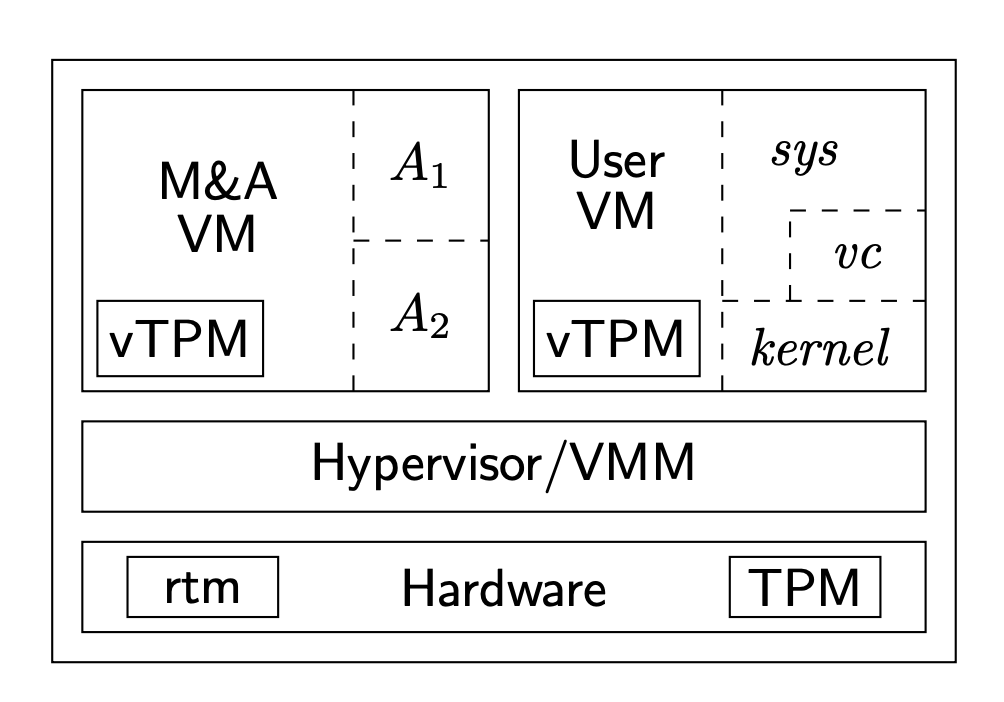
\includegraphics[scale=.5]{AttSystemRowe.png}
  \caption{An example attestation system defined by \cite{Rowe::Bundling}.}
  \label{att-system-rowe}
\end{figure}

Realizing this system, we can derive a bottom up measurement scheme which, taken from \cite{Rowe::Bundling}, can be visualized below. In this diagram, we propose that time begins at the top with the measurement of  the \emph{rtm}. This implies time flows downwards. In this notation, we consider a measurement event $ms_{ker}(vc,sys)$ imples the event of \emph{vc} measuring \emph{sys} in the context of \emph{ker}. Another example is $ms(rtm,A_1)$ where the measurement of $A_1$ is performed in the context of $rtm$. \todo{With this notation, I think contextual dependencies are represented as pairs}

\begin{figure}[hbtp]
  \centering
  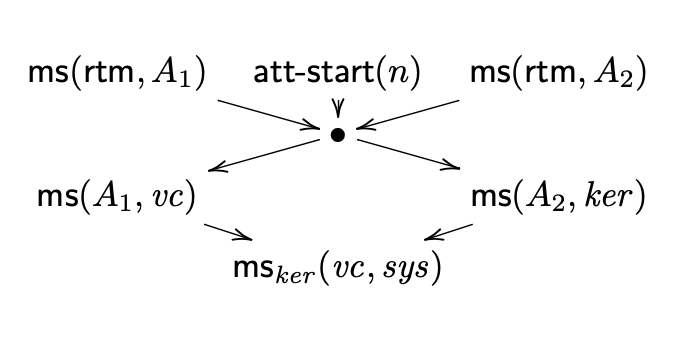
\includegraphics[scale=.5]{MeasOrdRowe.png}
  \caption{An example of measurement ordering from the previous system as defined by \cite{Rowe::Bundling}.}
  \label{meas-ord-rowe}
\end{figure}

So, now we have the set of \textbf{states} which are measurement events. The initial state is either some \textbf{rtm} (root of trust measurement) or some \textbf{att-start} event. THE TRANSITION RELATION THEN IS THE MEASUREMENT RELATION. 

Now, back to the example system presented in Figure \ref{fig:Host2}. We can represent this in a dependency like structure below similar to teh structure used by \cite{Rowe::Bundling}. 

\begin{figure}[hbtp]
  \centering
  \begin{tikzpicture}[->,>=stealth']

    \node[rectangle,
          draw,
          minimum width = 8cm, 
          minimum height = 6cm] (Host2) at (0,0) {};
    \node[anchor=south] at (Host2.south) {Host2}; 

    
    \node[rectangle,
    draw,
    dashed,
    fill = white,
    minimum width = 1cm, 
    minimum height = .75cm] (T2) at (0,2.25) {};
    \node at (T2.center) {T2};
    
    \node[rectangle,
    draw,
    fill = white,
    dashed,
    minimum width = 1.3cm, 
    minimum height = .75cm] (ASP2) at (-.15,1.25) {};
    \node at (ASP2.center) {ASP2};
    
    \node[rectangle,
        draw,
        minimum width = 4cm, 
        minimum height = 2cm] (MAVM) at (-1.5,1.75) {};
    \node[anchor=north west] at (MAVM.north west) {M$\&$A VM}; 
    
    \node[rectangle,
        draw,
        fill = white,
        minimum width = 7cm, 
        minimum height = 1cm] (VMM) at (0,0) {};
    \node[anchor=west] at (VMM.west) {VMM};

    \node[rectangle,
        draw,
        dashed,
        fill = white,
        minimum width = 1cm, 
        minimum height = .75cm] (OS) at (-1.5,0) {};
    \node at (OS.center) {OS};

    \node[rectangle,
        draw,
        dashed,
        fill = white,
        minimum width = 1cm, 
        minimum height = .75cm] (DR) at (0,0) {};
    \node at (DR.center) {DR};

    \node[rectangle,
        draw,
        fill = white,
        dashed,
        minimum width = 1cm, 
        minimum height = .75cm] (SIG) at (1.5,0) {};
    \node at (SIG.center) {$ \{ \}_{K}$};

    \node[rectangle,
        draw,
        fill = white,
        minimum width = 7cm, 
        minimum height = 1cm] (Hardware) at (0,-1.25) {};
    \node[anchor=west] at (Hardware.west) {Hardware};

    \node[rectangle,
        draw,
        dashed,
        fill = white,
        minimum width = 2cm, 
        minimum height = .75cm] (RoTM) at (0,-1.25) {};
    \node at (RoTM.center) {ROTM};

\end{tikzpicture}
  \caption{Host2 presented as one system.}
  \label{host2-block}
\end{figure}

We can then easily see how to create a transition system using the measures relation. 

\pagebreak

\bibliographystyle{acm}
\bibliography{citations.bib}

\end{document}